%%%%%%%%%%%%%%%%%%%%%%%%%%%%%%%%%%%%%%%%%
% Modelo para Projeto de trabalho de conclusão de curso
% Bacharelado em Sistemas de Informação - IFNMG - Campus Salinas
% Version 2 (1º semestre 2021)
%
% Modelo adaptado de:
% Frits Wenneker (http://www.howtotex.com)
%
% License:
% CC BY-NC-SA 3.0 (http://creativecommons.org/licenses/by-nc-sa/3.0/)
%
% Texto adaptado de: http://www.fea.usp.br/media/fck/File/Roteiro_para_projeto_pesquisa.pdf
%%%%%%%%%%%%%%%%%%%%%%%%%%%%%%%%%%%%%%%%%
\documentclass[
	% -- opções da classe memoir --
	12pt,				% tamanho da fonte
	%openright,			% capítulos começam em pág ímpar (insere página vazia caso preciso)
	twoside,			% para impressão em recto e verso. Oposto a oneside
	openany,			% capítulos começam na próxima página, sem inserir página em branco
	a4paper,			% tamanho do papel.
	% -- opções da classe abntex2 --
	chapter=TITLE,		% títulos de capítulos convertidos em letras maiúsculas
	section=TITLE,		% títulos de seções convertidos em letras maiúsculas
	subsection=TITLE,	% títulos de subseções convertidos em letras maiúsculas
	subsubsection=TITLE,% títulos de subsubseções convertidos em letras maiúsculas
	% -- opções do pacote babel --
	english,			% idioma adicional para hifenização
	french,				% idioma adicional para hifenização
	spanish,			% idioma adicional para hifenização
	brazil,				% o último idioma é o principal do documento
	]{abntex2}
% ---------------------------------
% PACOTES
% ---------------------------------
\renewcommand{\thesection}{\arabic{section}}
\usepackage{lmodern}			% Usa a fonte Latin Modern
\usepackage[T1]{fontenc}		% Selecao de codigos de fonte.
\usepackage[utf8]{inputenc}		% Codificacao do documento (conversão automática dos acentos)
\usepackage{indentfirst}		% Indenta o primeiro parágrafo de cada seção.
\usepackage{color}				% Controle das cores
\usepackage{graphicx}			% Inclusão de gráficos
\usepackage{microtype} 			% para melhorias de justificação
\usepackage{multirow}
\usepackage{amsmath,amsfonts,amssymb}
\usepackage[table]{xcolor}
\usepackage{multirow}           % Merge rows and columns in tables
\usepackage{longtable}          % Large tables
\usepackage{fancyvrb}           % Codes and Outputs commands
\usepackage{listings}           % Codes and Outputs commands
\usepackage{pdflscape}
\usepackage{float}
\usepackage{subfig}             % Subfigures
\usepackage{latexsym}           % Extra symbols of Latex
\usepackage{booktabs}
\usepackage{enumerate}
\usepackage{acronym}
\usepackage[portuguese, ruled, linesnumbered]{algorithm2e}
\usepackage[noend]{algpseudocode}
\usepackage{url}
\let\realurl\url
\renewcommand{\url}[1]{\realurl{#1}\wlog{URLX #1}}
\usepackage{lipsum}				% To generate dummy text
% ---------------------------------
% Pacotes de citações
% ---------------------------------
\usepackage[brazilian,hyperpageref]{backref}% Paginas com as citações na bibl
\usepackage[alf,bibjustif]{abntex2cite}	% Citações padrão ABNT
% ---------------------------------
% Configurações do pacote backref
% Usado sem a opção hyperpageref de backref
\renewcommand{\backrefpagesname}{Citado na(s) página(s):~}
% Texto padrão antes do número das páginas
\renewcommand{\backref}{}
% Define os textos da citação
\renewcommand*{\backrefalt}[4]{
	\ifcase #1 %
		Nenhuma citação no texto.%
	\or
		Citado na página #2.%
	\else
		Citado #1 vezes nas páginas #2.%
	\fi}%
% ---------------------------------
% Configurações de aparência do PDF final
% ---------------------------------
% alterando o aspecto da cor azul
\definecolor{blue}{RGB}{41,5,195}
% informações do PDF
\makeatletter
\hypersetup{
     	%pagebackref=true,
		pdftitle={\@title},
		pdfauthor={\@author},
    	pdfsubject={\imprimirpreambulo},
	    pdfcreator={LaTeX with abnTeX2},
		pdfkeywords={abnt}{latex}{abntex}{abntex2}{projeto de pesquisa},
		colorlinks=true,       		% false: boxed links; true: colored links
    	linkcolor=blue,          	% color of internal links
    	citecolor=blue,        		% color of links to bibliography
    	filecolor=magenta,      		% color of file links
		urlcolor=blue,
		bookmarksdepth=4
}
\makeatother
% ---------------------------------
% Espaçamentos entre linhas e parágrafos
% ---------------------------------
% O tamanho do parágrafo é dado por:
\setlength{\parindent}{1.3cm}
% Controle do espaçamento entre um parágrafo e outro:
\setlength{\parskip}{0.2cm}  % tente também \onelineskip
\raggedbottom                % evita esticar espaços para alinhar o fim das páginas
% ---------------------------------
%	SEÇÃO DE TÍTULO
% ---------------------------------
\newcommand{\horrule}[1]{\rule{\linewidth}{#1}}
\title{
\normalfont \normalsize
\textsc{Instituto Federal do Norte de Minas Gerais - Campus Salinas\\
        Bacharelado em Sistemas de Informação\\
        }
\horrule{2pt} \\[0.4cm]
\huge
        Sistema Web para Agendamento de Espaços Físicos no IFNMG -- Salinas \\
\horrule{2pt} \\[25pt]
}
\author{Aluno: Murilo Santos Gonçalves \\
[3mm]Orientador: Arthur Farias Porto\\
[3mm]Coorientadora: Jéssica Glória\\
}
\date{\normalsize\today}
% ---------------------------------
% Início do documento
% ---------------------------------
\begin{document}
% Seleciona o idioma do documento (conforme pacotes do babel)
\selectlanguage{brazil}
% Retira espaço extra obsoleto entre as frases.
\frenchspacing
% Imprimi a seção de títulos
\maketitle
\thispagestyle{empty}   % capa sem número de página
\clearpage              % a Introdução começa na página seguinte
\setcounter{page}{1}    % a capa não entra na contagem
%---------------------------------
% SEÇÃO DE INTRODUÇÃO
%---------------------------------
\section{Introdução}
\label{Introducao}
A organização dos espaços físicos num campus universitário pode aparentar simplicidade, mas revela-se complexa na prática. Quando laboratórios e salas especiais são compartilhados por vários docentes sem um sistema de agendamento adequado, surgem conflitos de horário e a tarefa de controlar quem usa o quê e quando recai sobre servidores que já têm outras atribuições.

No IFNMG -- Campus Salinas, esse problema tem contorno específico. O sistema utilizado para agendamentos exige que todos os horários já ocupados sejam cadastrados manualmente antes de qualquer reserva, um processo que precisa ser refeito a cada troca de semestre, uma vez que as atividades dos espaços variam significativamente ao longo do período letivo. Além do retrabalho contínuo, os docentes não têm autonomia para consultar disponibilidade ou solicitar reservas sem intermediação, e a instituição não dispõe de registro consolidado sobre a utilização dos laboratórios ao longo do tempo. Esse cenário não é exclusivo do Campus Salinas: estudo de \citeonline{cruz2023gestao} no IFNMG Campus Almenara identificou a ausência de planejamento permanente e de mecanismos para medir a utilização dos laboratórios.

Este trabalho propõe o desenvolvimento de um sistema web para o gerenciamento de reservas de espaços físicos no IFNMG -- Campus Salinas. A proposta visa permitir que docentes consultem a disponibilidade e realizem solicitações de reserva de forma autônoma, enquanto o servidor responsável pelos agendamentos acessa ferramentas de aprovação, recebe notificações e gera relatórios sobre o uso dos espaços.

Antes de optar pelo desenvolvimento de uma solução própria, foram investigadas alternativas já disponíveis no mercado e na comunidade de software livre, incluindo plataformas comerciais de reserva de espaços, como o Skedda \cite{skedda2025} e o Microsoft Bookings \cite{microsoft2025bookings}, além de sistemas acadêmicos desenvolvidos por outras instituições de ensino \cite{cruz2023gestao,nascimento2020reservas}. Essa investigação evidenciou que nenhuma dessas soluções atende ao requisito central apontado pela Direção de Ensino Técnico do campus: fazer com que a disponibilidade dos espaços reflita automaticamente a grade de horários institucional.

A necessidade de uma solução específica foi expressa pela Diretora de Ensino Técnico do IFNMG -- Campus Salinas, setor responsável pela gestão dos agendamentos, que destacou\footnote{Informação verbal fornecida pela Diretora de Ensino Técnico do IFNMG -- Campus Salinas, em reuniões remotas realizadas em julho de 2025, novembro de 2025 e abril de 2026.}:

\begin{citacao}
Precisamos de um software que forneça um mapa de utilização dos espaços do campus e permita que horários livres dos espaços sejam agendados pelos docentes, aprovados pelos administradores e visualizados por todos.
\end{citacao}

Espera-se que o sistema contribua para a otimização do uso dos espaços físicos, a redução de conflitos de agendamento e a melhoria na gestão institucional do campus.
%---------------------------------
% SEÇÃO DE OBJETIVOS
%---------------------------------
\subsection{Objetivo Geral}
\label{sec:objetivoGeral}
Desenvolver um sistema web para o gerenciamento de reservas de espaços físicos no IFNMG -- Campus Salinas.
\subsection{Objetivos Específicos}
\label{sec:objetivosEspecificos}
\begin{itemize}
    \item Levantar o processo atual de agendamento e identificar as necessidades dos perfis de usuários envolvidos;
    \item Especificar os requisitos funcionais e não funcionais do sistema;
    \item Planejar a implementação do sistema web, definindo as tecnologias e a arquitetura técnica a serem adotadas, com base nos requisitos especificados;
    \item Disponibilizar ao administrador ferramentas para a gestão dos agendamentos e o acompanhamento do uso dos espaços.
\end{itemize}
\subsection{Estrutura do Trabalho}
Este trabalho está estruturado da seguinte forma: no Capítulo 2 é apresentada a revisão bibliográfica, que abrange o contexto institucional, os trabalhos relacionados e a fundamentação tecnológica; no Capítulo 3, a metodologia utilizada na condução da pesquisa; no Capítulo 4, o cronograma de execução das etapas previstas; e, por fim, as referências bibliográficas consultadas.
%---------------------------------
% SEÇÃO DE REVISÃO
%---------------------------------
\section{Revisão Bibliográfica}
\label{sec:revbib}

Este capítulo apresenta o referencial teórico que embasa o problema e a solução propostos. A primeira parte situa o leitor no contexto institucional em que o problema ocorre: o IFNMG -- Campus Salinas e a forma como instituições de ensino lidam com a gestão de espaços físicos. A segunda parte apresenta os trabalhos relacionados, descrevendo iniciativas semelhantes já documentadas na literatura e identificando em que pontos o presente trabalho se distingue delas. A terceira parte reúne os conceitos técnicos que fundamentam o desenvolvimento do sistema web proposto, cobrindo engenharia de software, modelagem com UML, banco de dados, controle de acesso, arquitetura web, usabilidade e testes.

%-----------------------------------
\subsection{Contexto Institucional}
\label{sec:contexto}

Esta seção descreve o IFNMG -- Campus Salinas e o funcionamento dos seus espaços físicos e apresenta o que a literatura registra sobre gestão de espaços em ambientes acadêmicos.

%-----------------------------------
\subsubsection{O IFNMG e o Campus Salinas}
\label{sec:ifnmg}

O Instituto Federal de Educação, Ciência e Tecnologia do Norte de Minas Gerais (IFNMG) é uma autarquia federal criada pela Lei n.º 11.892, de 29 de dezembro de 2008, que reorganizou a Rede Federal de Educação Profissional, Científica e Tecnológica no Brasil. Conforme seu Plano de Desenvolvimento Institucional, o IFNMG tem por missão promover educação profissional, científica e tecnológica por meio do ensino, da pesquisa e da extensão, com vistas à formação humana integral e ao desenvolvimento regional \cite{ifnmg2024pdi}.

O Campus Salinas integra a rede do IFNMG e oferta cursos em diferentes níveis e modalidades, entre eles o Bacharelado em Sistemas de Informação, no âmbito do qual este trabalho está inserido. Para o funcionamento dessas atividades acadêmicas, o campus dispõe de laboratórios de informática e outras salas especiais cujo uso é compartilhado por diferentes turmas e docentes ao longo do período letivo, o que exige mecanismos de organização e controle sobre a ocupação desses espaços.

A natureza dos institutos federais agrava esse desafio. Ao contrário de instituições que ofertam um único tipo de curso, os IFs atendem simultaneamente a turmas de educação técnica integrada ao ensino médio, cursos técnicos subsequentes e cursos de nível superior, todos com horários distintos e, em muitos casos, disputando os mesmos laboratórios. Um laboratório de informática, por exemplo, pode ser utilizado em horários diferentes para aulas de disciplinas técnicas, para disciplinas do bacharelado e para atividades de extensão, o que torna a gestão manual da disponibilidade um trabalho de complexidade operacional \cite{ifnmg2024pdi}.

%-----------------------------------
\subsubsection{A Gestão de Espaços em Instituições de Ensino}
\label{sec:gestao}

A gestão dos espaços físicos em instituições de ensino inclui o planejamento do uso, o controle de disponibilidade, o registro de ocupações e o acompanhamento de como os recursos são efetivamente utilizados. Quando esses mecanismos não existem ou são precários, o resultado é a subutilização dos espaços e a dificuldade de responder a demandas concretas dos usuários.

Esse cenário se repete em outras instituições públicas de ensino, como mostram os trabalhos de \citeonline{cruz2023gestao} e \citeonline{nascimento2020reservas}, discutidos na Seção~\ref{sec:trabrel}.

%-----------------------------------
\subsection{Trabalhos Relacionados}
\label{sec:trabrel}

Esta seção apresenta trabalhos e soluções que trataram de problemas semelhantes ao abordado nesta pesquisa, seja pelo diagnóstico da gestão de espaços em instituições federais de ensino, seja pelo desenvolvimento de sistemas de reserva em ambientes acadêmicos, seja pela oferta de ferramentas de mercado para a reserva de espaços. A análise desses trabalhos e soluções permite situar a presente proposta em relação ao que já foi produzido e identificar os aspectos que a diferenciam.

%-----------------------------------
\subsubsection{Soluções Existentes de Reserva de Espaços}
\label{sec:relsoftwares}

Além dos trabalhos acadêmicos, foram analisadas soluções de software já disponíveis para a reserva de espaços, com o objetivo de verificar se alguma delas resolveria o problema do Campus Salinas sem a necessidade de desenvolvimento de um sistema específico. A análise concentrou-se em duas plataformas comerciais representativas: o Skedda e o Microsoft Bookings.

O Skedda é uma plataforma web dedicada à reserva de espaços físicos, como salas, escritórios e laboratórios, que oferece autoatendimento aos usuários, definição de regras de reserva e visualização de disponibilidade em formato de agenda \cite{skedda2025}. O Microsoft Bookings, integrante do pacote Microsoft 365, é voltado ao agendamento de compromissos e ao gerenciamento de calendários, com reserva de recursos por meio de caixas de correio associadas a salas \cite{microsoft2025bookings}. Ambas as ferramentas cobrem funcionalidades que também são esperadas do sistema proposto, como a consulta de disponibilidade, a solicitação de reserva pelo próprio usuário e a notificação automática das partes envolvidas, o que demonstra a maturidade desse tipo de aplicação no mercado.

Nenhuma das duas, contudo, resolve o problema central do campus: fazer a disponibilidade refletir a grade de horários institucional. Como não importam as planilhas de horários, a ocupação das aulas teria de ser cadastrada manualmente a cada semestre, exatamente o retrabalho que motiva esta proposta. Além disso, são soluções proprietárias, pagas por assinatura e hospedadas em servidores externos, o que gera custos recorrentes e reduz o controle da instituição sobre os próprios dados.

%-----------------------------------
\subsubsection{Gestão de Laboratórios no IFNMG Campus Almenara}
\label{sec:relcaio1}

\citeonline{cruz2023gestao} conduziram uma pesquisa de campo no IFNMG Campus Almenara com o objetivo de analisar a utilização dos espaços e equipamentos dos laboratórios educacionais daquela unidade. O estudo adotou abordagem qualitativa e quantitativa, com coleta de dados por meio de questionários aplicados a servidores e docentes do campus. Os resultados revelaram que a gestão dos laboratórios ocorre de forma informal, baseada exclusivamente em reservas pontuais feitas com antecedência, sem planejamento oficial permanente e sem qualquer mecanismo para medir o desempenho ou a eficiência no uso desses espaços.

O trabalho de \citeonline{cruz2023gestao} contribui para a presente pesquisa ao documentar, em um campus do próprio IFNMG, a mesma ausência de ferramentas de gestão identificada no Campus Salinas. A semelhança entre os dois contextos reforça que o problema não é localizado e que a carência de soluções tecnológicas adequadas é uma realidade institucional mais ampla. No entanto, o trabalho desses autores se limita ao diagnóstico: não propõe nem desenvolve qualquer solução de software para o problema identificado. O presente trabalho avança nessa direção ao propor um sistema que automatiza o controle de disponibilidade e registra o histórico de uso dos espaços.

%-----------------------------------
\subsubsection{Sistema Web de Reservas na UESPI -- Parnaíba}
\label{sec:relcaio2}

\citeonline{nascimento2020reservas} desenvolveram um sistema web para controlar pedidos de reservas de recursos físicos na Universidade Estadual do Piauí, Campus Parnaíba. O contexto era semelhante ao do presente trabalho: as reservas de espaços e equipamentos eram registradas manualmente por servidores em uma agenda digital, e a demanda tornava o processo oneroso e sujeito a falhas. A solução desenvolvida pelos autores automatizou o controle das solicitações, disponibilizou a interface para os usuários da instituição e obteve avaliação positiva quanto à satisfação dos usuários com o sistema.

O trabalho de \citeonline{nascimento2020reservas} demonstra que o desenvolvimento de sistemas web de reserva em instituições de ensino é viável e resulta em ganhos concretos para a gestão. A presente proposta compartilha o mesmo problema central, mas apresenta características que a diferenciam. A principal delas é a importação das planilhas de horários institucionais, com reimportação ou ajuste pontual ao longo do semestre. Além disso, oferece consulta pública da ocupação, sem autenticação, e relatórios de uso dos espaços, recursos não descritos no trabalho referenciado. A Tabela~\ref{tab:comparativo} resume essa comparação.

\begin{table}[!htb]
	\centering
	\caption{Comparação entre o sistema proposto e os trabalhos relacionados}
	\begin{tabular}{@{}>{\raggedright\arraybackslash}p{5.6cm}cccc@{}}
	\hline
		\textbf{Funcionalidade} & \textbf{Skedda} & \textbf{\begin{tabular}[c]{@{}c@{}}MS\\ Bookings\end{tabular}} & \textbf{\begin{tabular}[c]{@{}c@{}}Nascimento, Rios\\ e Baluz (2020)\end{tabular}} & \textbf{\begin{tabular}[c]{@{}c@{}}Este\\ trabalho\end{tabular}} \\ \hline
		Solicitação de reserva pelo próprio usuário & $\checkmark$ & $\checkmark$ & $\checkmark$ & $\checkmark$ \\
		Aprovação das solicitações & $\checkmark$ & P & $\checkmark$ & $\checkmark$ \\
		Notificações automáticas & $\checkmark$ & $\checkmark$ & $\checkmark$ & $\checkmark$ \\
		Consulta pública, sem login & $\checkmark$ & P & $\times$ & $\checkmark$ \\
		Importação da grade de horários institucional & $\times$ & $\times$ & $\times$ & $\checkmark$ \\
		Relatórios de uso dos espaços & $\checkmark$ & $\checkmark$ & -- & $\checkmark$ \\
		Sem custo de assinatura & $\times$ & $\times$ & $\checkmark$ & $\checkmark$ \\ \hline
	\end{tabular}
	\caption*{\footnotesize Legenda: $\checkmark$ atende; P atende parcialmente; $\times$ não atende; -- não informado. \citeonline{cruz2023gestao} não constam por se tratar de estudo diagnóstico, sem sistema desenvolvido.\\ Fonte: Elaborado pelo autor (2026).}
	\label{tab:comparativo}
\end{table}

%-----------------------------------
\subsection{Fundamentação Tecnológica}
\label{sec:fundtec}

Esta seção apresenta os conceitos técnicos que embasam o sistema proposto: engenharia de software, UML, banco de dados, controle de acesso, arquitetura web, o \textit{framework} Django, usabilidade e testes.

%-----------------------------------
\subsubsection{Engenharia de Software}
\label{sec:engsw}

\citeonline{sommerville2018} define software como programas de computador e documentação associada, que pode ser desenvolvido para um cliente específico ou para o mercado em geral. A engenharia de software é a disciplina que se ocupa de todos os aspectos da produção de software, desde a especificação inicial do sistema até as necessidades de manutenção após a sua implantação. Deste campo, este trabalho se apoia diretamente em dois pontos: a especificação de requisitos e os atributos de qualidade que orientam as decisões de projeto.

Um conceito central dessa disciplina é a especificação de requisitos. \citeonline{sommerville2018} distingue os requisitos funcionais dos não funcionais: os primeiros descrevem as funções que o sistema deve executar e como deve se comportar em situações específicas; os segundos estabelecem restrições ao sistema, como desempenho, segurança e disponibilidade.

\citeonline{sommerville2018} também descreve atributos que um sistema de software profissional precisa apresentar para ser considerado de boa qualidade: manutenibilidade, ou seja, a capacidade de evoluir para atender a necessidades futuras; confiabilidade e segurança, que inclui comportamento correto e proteção contra falhas e acessos indevidos; eficiência, que diz respeito ao uso criterioso dos recursos de hardware; e aceitabilidade, que significa ser compreensível e compatível com o que os usuários esperam.

%-----------------------------------
\subsubsection{Modelagem de Sistemas com UML}
\label{sec:uml}

A \textit{Unified Modeling Language} (UML) é uma linguagem de modelagem padronizada para especificar, visualizar e documentar sistemas de software orientados a objetos \cite{bezerra2007}. \citeonline{bezerra2007} esclarece que a UML não é uma metodologia de desenvolvimento, mas uma notação que pode ser adotada em conjunto com diferentes processos. Ela oferece um conjunto de diagramas que representam aspectos distintos do sistema, como a sua estrutura estática e o seu comportamento dinâmico.

Entre os diagramas oferecidos pela UML, três são amplamente utilizados na modelagem de sistemas de informação. O diagrama de casos de uso descreve as funcionalidades do sistema do ponto de vista de quem interage com ele: representa os atores (usuários ou sistemas externos), os casos de uso (as funções que o sistema oferece) e os relacionamentos entre eles, delimitando o escopo funcional do sistema sem detalhar como cada função é implementada. O diagrama de classes representa a estrutura estática do sistema, descrevendo as classes do domínio, seus atributos, métodos e os relacionamentos entre elas, como associação, herança e agregação; é o diagrama mais próximo da estrutura do código. O diagrama de sequência representa o comportamento dinâmico do sistema, mostrando a troca de mensagens entre os objetos ao longo do tempo para a realização de um processo específico, o que permite visualizar a ordem das interações e os pontos de decisão de um fluxo \cite{larman2007}.

\citeonline{larman2007} destaca que a modelagem com UML permite registrar e comunicar decisões de projeto de forma visual antes de qualquer implementação, o que facilita o alinhamento entre desenvolvedores e demais partes envolvidas.
%-----------------------------------
\subsubsection{Banco de Dados Relacional}
\label{sec:bd}

Um banco de dados é uma coleção organizada de dados inter-relacionados, gerenciada por um sistema que permite armazená-los, recuperá-los e manipulá-los com eficiência \cite{heuser2009}. \citeonline{heuser2009} apresenta o modelo entidade-relacionamento como a principal ferramenta para o projeto conceitual de bancos de dados, por permitir representar as entidades do domínio e os vínculos entre elas antes de definir como os dados serão fisicamente armazenados.

O modelo relacional organiza os dados em tabelas formadas por linhas e colunas, onde cada tabela representa uma entidade e cada linha, um registro dessa entidade. A integridade dos dados é assegurada por restrições como chaves primárias e estrangeiras, que garantem a unicidade dos registros e os vínculos entre tabelas \cite{silberschatz2012}. \citeonline{heuser2009} também descreve o processo de normalização, pelo qual o esquema relacional é reorganizado para eliminar redundâncias e anomalias de atualização. Um banco de dados normalizado garante que cada informação seja armazenada em um único lugar, reduzindo o risco de inconsistências quando os dados precisam ser modificados.

\citeonline{silberschatz2012} definem um sistema gerenciador de banco de dados (SGBD) como um conjunto de programas que permite criar, manter e acessar um banco de dados. Os autores também descrevem a linguagem SQL (\textit{Structured Query Language}) como o padrão para definir esquemas, inserir dados e realizar consultas em bancos de dados relacionais. A SQL combina uma linguagem de definição de dados, para criar e alterar tabelas e restrições, com uma linguagem de manipulação de dados, para inserir, atualizar, remover e consultar registros. Para o sistema proposto, o uso de um SGBD relacional é adequado porque os dados a serem gerenciados (espaços físicos, horários, usuários, solicitações de reserva) têm estrutura bem definida e mantêm entre si relacionamentos que o modelo relacional representa com precisão.

Entre os SGBDs relacionais disponíveis, o PostgreSQL é um sistema de código aberto com mais de três décadas de desenvolvimento, reconhecido pela conformidade com o padrão SQL e pela robustez no tratamento de transações. Ele garante as propriedades ACID (atomicidade, consistência, isolamento e durabilidade), oferece suporte a tipos de dados avançados, controle de concorrência multiversão (MVCC) e recursos como busca textual e integridade referencial, características que o tornam adequado a aplicações que exigem consistência e confiabilidade no armazenamento dos dados \cite{postgresql2024}.

%-----------------------------------
\subsubsection{Controle de Acesso Baseado em Papéis}
\label{sec:rbac}

O controle de acesso define quais usuários têm permissão para executar quais operações em um sistema. Entre os modelos existentes, o \textit{Role-Based Access Control} (RBAC) proposto por \citeonline{sandhu1996rbac} é amplamente adotado em sistemas de informação institucionais.

No modelo RBAC, os direitos de acesso são associados a papéis, e os usuários adquirem esses direitos ao serem atribuídos a um ou mais papéis. \citeonline{sandhu1996rbac} descrevem que essa abordagem simplifica a administração, pois as permissões são definidas no nível do papel e não para cada usuário individualmente. Quando as responsabilidades de um usuário mudam, basta alterar a sua atribuição de papéis, sem necessidade de revisar cada permissão específica.

\citeonline{sandhu1996rbac} definem quatro modelos de referência que compõem a família RBAC. O RBAC0, o modelo base, define os elementos fundamentais: usuários, papéis, permissões e sessões, onde uma sessão corresponde a um período de atividade de um usuário dentro de um subconjunto dos seus papéis. O RBAC1 estende o modelo base com hierarquias de papéis, permitindo que papéis mais abrangentes herdem as permissões de papéis subordinados. O RBAC2 acrescenta restrições ao RBAC0, incluindo o conceito de separação de obrigações, pelo qual um usuário não pode acumular simultaneamente papéis conflitantes. O RBAC3 combina hierarquias e restrições, reunindo as características dos modelos anteriores.

O sistema proposto segue o RBAC0 com restrições típicas do RBAC2, sem hierarquia de papéis. As restrições adotadas são a cardinalidade, pela qual cada usuário tem no máximo um perfil, e a reserva de permissões administrativas, que não podem ser atribuídas a nenhum perfil. No padrão NIST para RBAC, essa configuração corresponde ao \textit{Core RBAC} com restrição de cardinalidade \cite{ferraiolo2001nist}. Como cada usuário tem um único perfil, a separação de obrigações entre papéis conflitantes não se aplica.

Duas regras do sistema complementam o modelo por papéis. A primeira trata de quem pode atribuir perfis: um usuário só atribui um perfil se já tiver todas as permissões dele, questão estudada pelo RBAC administrativo \cite{sandhu1999arbac97}. A segunda considera o vínculo do usuário com o registro, e não só o perfil: o docente de uma aula pode cancelar as ocorrências dela, e disciplinas e turmas ficam limitadas ao escopo do docente. Esse tipo de verificação se aproxima do controle por atributos, combinado ao RBAC em modelos híbridos \cite{kuhn2010attributes}.

%-----------------------------------
\subsubsection{Desenvolvimento Web e Arquitetura de Software}
\label{sec:web}

Um sistema web é uma aplicação de software acessada por meio de um navegador, que utiliza a infraestrutura da internet para a comunicação entre clientes e servidores. \citeonline{tanenbaum2011} descrevem a \textit{World Wide Web} como um sistema de documentos interconectados distribuídos pela internet, baseado no protocolo HTTP para a troca de informações. Esse modelo de comunicação é a base sobre a qual sistemas web são construídos.

Do ponto de vista arquitetural, \citeonline{laudon2014} descrevem que sistemas de informação baseados na web se organizam tipicamente em três camadas: a de apresentação, responsável pela interface com o usuário no navegador; a de aplicação, onde ficam as regras de negócio; e a de dados, onde as informações são armazenadas. Essa separação em camadas facilita a manutenção e permite que cada parte do sistema seja modificada sem afetar diretamente as demais.

\citeonline{tanenbaum2011} descrevem o protocolo HTTP como uma especificação sem estado (\textit{stateless}), o que significa que cada requisição do cliente ao servidor é tratada de forma independente, sem que o servidor retenha informações sobre interações anteriores. Essa característica simplifica a arquitetura dos servidores web, mas exige que o estado da aplicação, como a sessão do usuário autenticado, seja gerenciado explicitamente pela camada de aplicação, por meio de mecanismos como \textit{tokens} de autenticação.

\citeonline{laudon2014} também apontam que sistemas web têm a vantagem de não exigir instalação de software no dispositivo do usuário: basta um navegador com acesso à internet para que o sistema esteja disponível. Isso reduz os custos de implantação, elimina problemas de compatibilidade entre sistemas operacionais e centraliza a manutenção no servidor, onde atualizações passam a valer imediatamente para todos os usuários. No caso do sistema proposto, essa característica é relevante porque os docentes do campus utilizam dispositivos variados e não dependem de nenhuma configuração específica para acessar a plataforma de reservas.

Para o sistema proposto, a arquitetura em três camadas é adequada porque isola a interface utilizada pelos docentes da lógica que controla as reservas e da base de dados onde os registros são mantidos. Na prática, essa separação é implementada por meio de um \textit{framework} web, que fornece a estrutura de código e os mecanismos de comunicação entre as camadas, reduzindo o trabalho de infraestrutura e permitindo que o desenvolvimento se concentre nas regras de negócio da aplicação. O padrão arquitetural adotado pelo \textit{framework} escolhido para este sistema é detalhado na seção a seguir.

%-----------------------------------
\subsubsection{Padrões Arquiteturais para Aplicações Web: MVC e MTV}
\label{sec:mvc_mtv}

O padrão \textit{Model-View-Controller} (MVC) é uma abordagem arquitetural consolidada para organizar o código de aplicações interativas em três componentes com responsabilidades bem delimitadas. O \textit{Model} gerencia os dados e as regras de negócio da aplicação. A \textit{View} é responsável pela apresentação das informações ao usuário. O \textit{Controller} recebe as ações do usuário, processa as entradas e coordena a interação entre \textit{Model} e \textit{View} \cite{djangodocs}. Essa separação permite que cada componente seja desenvolvido e testado de forma independente.

O \textit{framework} Django adota uma variação desse padrão denominada MTV (\textit{Model-Template-View}), que redistribui as responsabilidades de forma distinta. O \textit{Model} cumpre a mesma função do MVC: representa as entidades de dados e encapsula as regras de negócio associadas ao banco de dados. O \textit{Template} substitui a \textit{View} do MVC e se ocupa exclusivamente da renderização da interface, gerando o HTML entregue ao navegador. A \textit{View} do MTV, por sua vez, assume o papel que no MVC pertenceria ao \textit{Controller}: ela recebe a requisição HTTP, aciona os \textit{Models} necessários e seleciona o \textit{Template} adequado para compor a resposta \cite{treinaweb2023mtv}. A Figura~\ref{fig:mtv} ilustra essa organização.

\begin{figure}[!htb]
    \centering
    \caption{Arquitetura MTV do Django}
    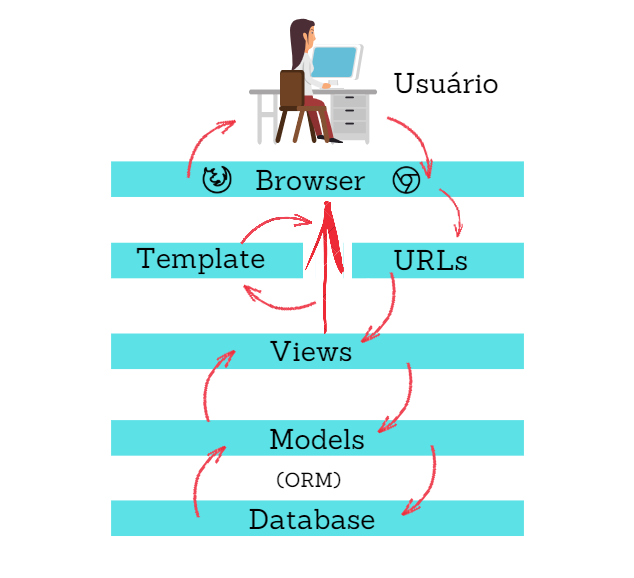
\includegraphics[width=0.85\textwidth]{Figuras/mvt-django.png}
    \caption*{Fonte: \cite{treinaweb2023mtv}}
    \label{fig:mtv}
\end{figure}

A diferença mais relevante entre os dois padrões está na forma como o roteamento de requisições é gerenciado. No MVC clássico, o \textit{Controller} é o ponto de entrada das requisições do cliente. No MTV do Django, esse papel é desempenhado pelo próprio mecanismo de roteamento de URLs do \textit{framework}, que mapeia cada endereço recebido para a \textit{View} correspondente por meio do arquivo \texttt{urls.py}, antes mesmo de qualquer lógica da aplicação ser acionada \cite{djangodocs}. A Figura~\ref{fig:mvc-vs-mtv} compara os dois padrões.

\begin{figure}[!htb]
    \centering
    \caption{Comparação entre as arquiteturas MVC e MTV}
    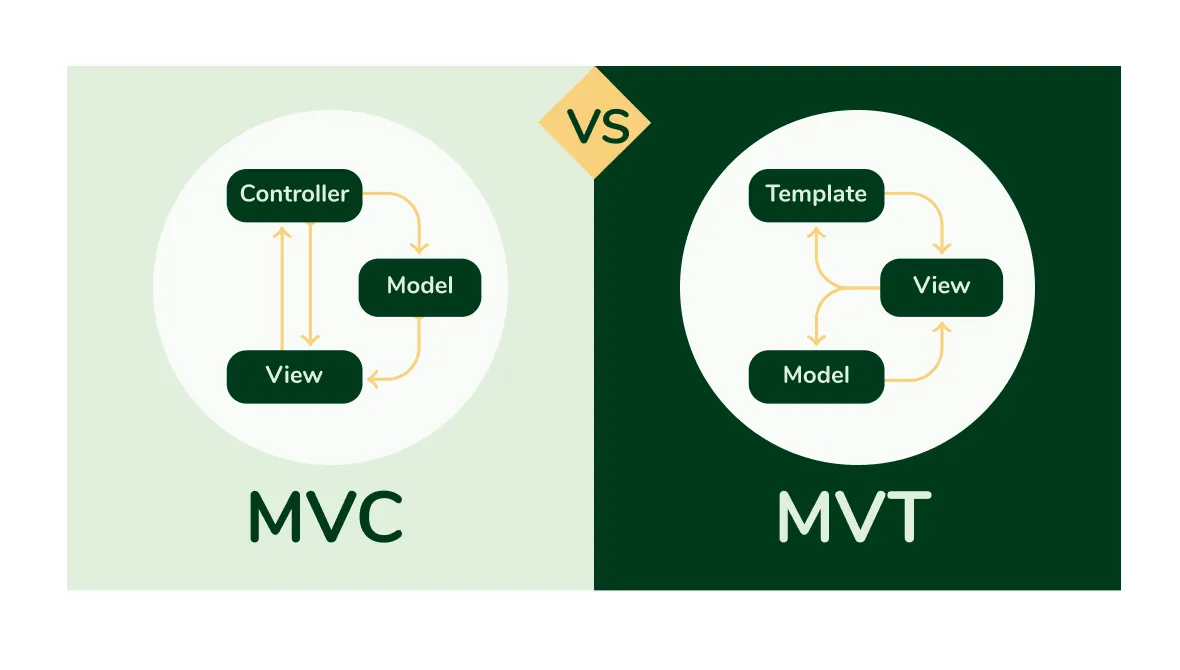
\includegraphics[width=0.85\textwidth]{Figuras/mvcVSmvt.png}
    \caption*{Fonte: \cite{djangodocs}}
    \label{fig:mvc-vs-mtv}
\end{figure}

O fluxo de uma requisição no Django, representado na Figura~\ref{fig:fluxo-mtv}, percorre essas camadas de forma sequencial: o cliente envia uma requisição HTTP, o roteador de URLs identifica a \textit{View} responsável, a \textit{View} acessa os \textit{Models} para obter ou persistir dados e, em seguida, seleciona o \textit{Template} adequado para gerar a resposta enviada de volta ao cliente \cite{silva2023mtv}.

\begin{figure}[!htb]
    \centering
    \caption{Fluxo de requisição na arquitetura MTV do Django}
    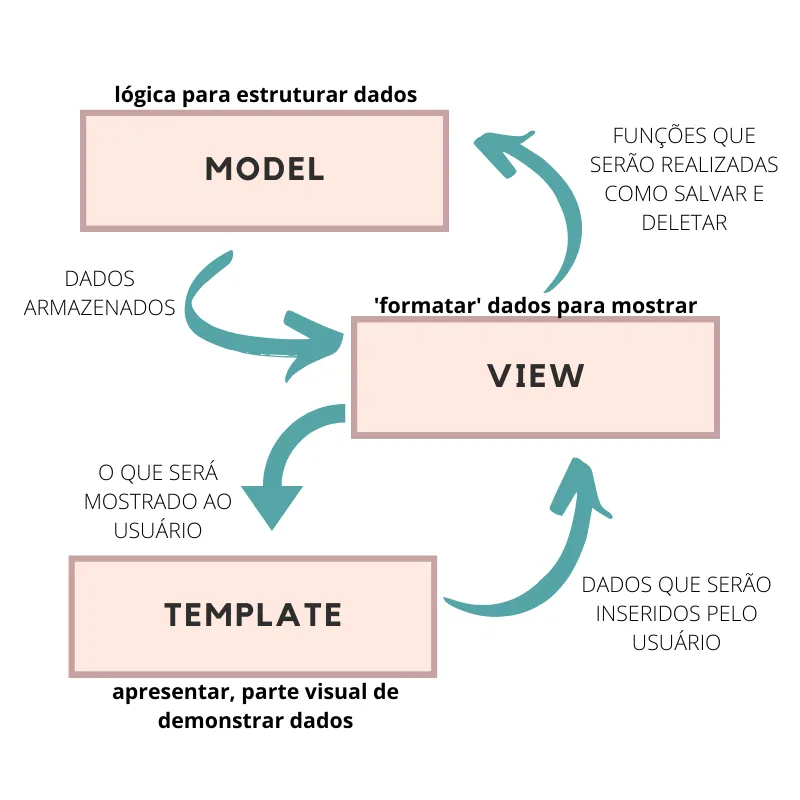
\includegraphics[width=0.85\textwidth]{Figuras/arquitetura.png}
    \caption*{Fonte: \cite{silva2023mtv}}
    \label{fig:fluxo-mtv}
\end{figure}

%-----------------------------------
\subsubsection{O Framework Django}
\label{sec:django}

O Django é um \textit{framework} web de código aberto escrito em Python. Ele opera segundo o princípio \textit{batteries included}: disponibiliza nativamente os componentes mais comuns no desenvolvimento web, como ORM, sistema de autenticação, roteamento de URLs, mecanismo de \textit{templates} e envio de e-mails, sem dependência de bibliotecas externas para essas funções \cite{djangodocs}. Outro princípio central do \textit{framework} é o \textit{Don't Repeat Yourself} (DRY), que orienta o reaproveitamento de código e a centralização de lógicas que, se duplicadas, aumentariam o custo de manutenção ao longo do tempo \cite{djangodocs}.

O roteamento de URLs é configurado no arquivo \texttt{urls.py}, que associa cada padrão de endereço a uma \textit{view} específica por meio da função \texttt{path()}. Quando uma requisição chega ao servidor, o \textit{framework} percorre a lista de padrões registrados até encontrar o primeiro que corresponda à URL solicitada e delega o processamento à \textit{view} associada. Esse mecanismo é independente da estrutura de diretórios da aplicação, o que permite organizar as URLs de forma legível e separada da lógica de negócio \cite{djangodocs}.

Cada \textit{model} do Django é uma classe Python que herda de \texttt{django.db.models.Model}. Cada atributo da classe representa uma coluna da tabela correspondente no banco de dados, e o tipo do campo, como \texttt{CharField}, \texttt{DateTimeField} ou \texttt{BooleanField}, determina o tipo de dado armazenado e as validações aplicadas \cite{djangodocs}. Relacionamentos entre entidades são representados por campos específicos: \texttt{ForeignKey} para associações muitos-para-um e \texttt{ManyToManyField} para associações muitos-para-muitos. O ORM traduz as operações sobre esses objetos Python em comandos SQL compatíveis com o banco de dados configurado \cite{djangodocs}.

As mudanças nos \textit{models} são controladas pelo sistema de \textit{migrations}. O comando \texttt{makemigrations} gera um arquivo descrevendo as alterações a serem aplicadas no banco; o comando \texttt{migrate} as aplica de forma incremental e rastreável, mantendo um histórico completo de todas as versões do esquema \cite{djangodocs}.

O sistema de \textit{templates} do Django utiliza a \textit{Django Template Language} (DTL), que insere dados dinâmicos nas páginas HTML por meio de variáveis e \textit{tags} de controle. A herança de \textit{templates}, obtida com as \textit{tags} \texttt{\{\% extends \%\}} e \texttt{\{\% block \%\}}, permite que um \textit{template} base defina a estrutura comum a todas as páginas, como cabeçalho, menu e rodapé, e que os demais \textit{templates} sobrescrevam apenas os blocos de conteúdo específicos \cite{djangodocs}. Esse recurso elimina duplicação de HTML e garante consistência visual em toda a aplicação.

O Django oferece proteções de segurança ativas por padrão. A proteção contra \textit{Cross-Site Request Forgery} (CSRF) é implementada por um \textit{middleware} que exige um \textit{token} válido em todas as requisições que modificam dados no servidor; a \textit{tag} \texttt{\{\% csrf\_token \%\}} insere esse \textit{token} automaticamente nos formulários. A proteção contra \textit{Cross-Site Scripting} (XSS) é garantida pelo sistema de \textit{templates}, que escapa automaticamente todo conteúdo dinâmico antes de inseri-lo no HTML. A proteção contra injeção de SQL é inerente ao ORM, que parametriza internamente as consultas geradas, de modo que dados fornecidos pelo usuário nunca são interpolados diretamente no SQL \cite{djangodocs}.


%-----------------------------------
\subsubsection{Usabilidade e Interface do Usuário}
\label{sec:usab}

Usabilidade é a medida em que um produto pode ser usado por pessoas específicas para atingir objetivos específicos com eficácia, eficiência e satisfação num determinado contexto \cite{nielsen1993}. \citeonline{nielsen1993} descreve cinco atributos que compõem a usabilidade de um sistema: facilidade de aprendizado, eficiência de uso, facilidade de memorização, baixa taxa de erros e satisfação subjetiva do usuário. Um sistema com boa usabilidade permite que o usuário realize suas tarefas sem depender de treinamento extensivo nem de suporte constante.

Para orientar o projeto de interfaces, \citeonline{nielsen1994} propôs dez heurísticas de usabilidade que se tornaram referência na área: (1) visibilidade do estado do sistema, mantendo o usuário informado sobre o que está acontecendo; (2) correspondência entre o sistema e o mundo real, usando linguagem e convenções familiares ao usuário; (3) controle e liberdade do usuário, permitindo desfazer ações e sair de estados indesejados; (4) consistência e padrões, seguindo convenções da plataforma para que o usuário não precise aprender novos significados; (5) prevenção de erros, projetando para evitar que erros ocorram; (6) reconhecimento em vez de memorização, tornando objetos e opções visíveis para reduzir a carga de memória do usuário; (7) flexibilidade e eficiência de uso, permitindo que usuários experientes realizem tarefas mais rapidamente; (8) estética e design minimalista, evitando informações irrelevantes que competem com o conteúdo principal; (9) ajuda para reconhecer, diagnosticar e recuperar erros, exibindo mensagens claras sobre o que deu errado e como corrigir; e (10) ajuda e documentação, oferecendo suporte quando necessário, de forma fácil de buscar e orientada à tarefa.

Algumas dessas heurísticas têm peso particular no sistema proposto. A visibilidade do estado do sistema é importante porque o docente precisa saber, a qualquer momento, se a sua solicitação de reserva está pendente, aprovada ou rejeitada. A correspondência com o mundo real orienta o uso de termos como ``laboratório'', ``reserva'' e ``disponível'' em vez de jargões técnicos. A prevenção de erros, por sua vez, inclui mecanismos como a verificação automática de conflitos de horário antes de permitir a solicitação.

No contexto deste trabalho, usabilidade é relevante porque o sistema será utilizado por docentes com familiaridade tecnológica variada. Um sistema que exija treinamento extensivo ou que gere dúvidas frequentes tende a ser abandonado, o que comprometeria o próprio objetivo de substituir o processo manual de agendamento.
%-----------------------------------
\subsubsection{Testes de Software}
\label{sec:testes}

Testes de software são atividades planejadas com o objetivo de verificar se um sistema se comporta conforme o esperado e identificar defeitos antes que o produto chegue ao usuário final. \citeonline{sommerville2018} define teste como um processo de validação e verificação que busca demonstrar que o software atende aos seus requisitos e identificar situações em que ele se comporta de forma incorreta ou inesperada. \citeonline{pressman2016} complementam essa perspectiva ao afirmar que testar é executar um programa com a intenção explícita de encontrar erros, distinguindo o processo de testes de outras atividades de garantia de qualidade por seu caráter sistematicamente verificativo: um teste bem-sucedido é aquele que revela um defeito até então desconhecido.

Os testes unitários são a forma mais elementar de teste de software e têm como foco verificar o comportamento de unidades individuais de código de forma isolada, antes de integrá-las ao restante do sistema. \citeonline{myers2011} definem teste unitário como o processo de testar subprogramas, funções ou métodos de maneira independente, de modo que, quando uma unidade falha, a localização do defeito seja imediata, sem a necessidade de investigar interações entre múltiplos componentes. \citeonline{pressman2016} acrescentam que os testes unitários devem cobrir as estruturas de controle internas de cada componente, as condições de contorno, os caminhos independentes de execução e o tratamento de erros.

No contexto de sistemas web com regras de negócio definidas, os testes unitários têm papel direto na validação da lógica da aplicação. \citeonline{sommerville2018} observa que os testes unitários são especialmente eficazes para validar componentes que implementam regras de negócio, pois permitem verificar cada condição individualmente e com precisão. À medida que as unidades validadas são combinadas, os testes de integração verificam se os componentes interagem corretamente entre si \cite{pressman2016}.

%---------------------------------
% SEÇÃO DE METODOLOGIA
%---------------------------------
\section{Metodologia}
\label{sec:metodologia}

Este capítulo descreve a metodologia da pesquisa. A Seção~\ref{sec:tipopesquisa} classifica a pesquisa quanto à natureza, aos objetivos e ao procedimento técnico, e a Seção~\ref{sec:procedimentos} descreve as etapas do trabalho.

%-----------------------------------
\subsection{Tipo de Pesquisa}
\label{sec:tipopesquisa}

Quanto à natureza, esta pesquisa é aplicada. Sua finalidade é produzir um artefato de software para um problema concreto identificado num contexto institucional real, não ampliar o conhecimento teórico de forma genérica. \citeonline{gil2008} distingue a pesquisa aplicada da pesquisa básica precisamente por esse critério: a primeira é motivada pela necessidade de resolver problemas práticos e seus resultados têm aplicação imediata.

Quanto aos objetivos, a pesquisa é descritiva. O ponto de partida é a caracterização do processo atual de agendamento de espaços físicos no IFNMG -- Campus Salinas: como ele funciona, onde falha e o que os usuários envolvidos precisam que mude. \citeonline{gil2008} define a pesquisa descritiva como aquela que busca descrever as características de determinado fenômeno e estabelecer relações entre suas variáveis, sem que o pesquisador interfira nos fatos observados.

Quanto ao procedimento técnico, a pesquisa adota o estudo de caso em combinação com pesquisa bibliográfica. O estudo de caso é adequado porque a investigação recai sobre um ambiente específico, o Campus Salinas, com histórico, atores e restrições próprios que precisam ser compreendidos antes de qualquer proposta de solução. \citeonline{yin2015} define o estudo de caso como uma investigação empírica que examina um fenômeno contemporâneo em profundidade e em seu contexto real, sendo especialmente indicado quando os limites entre o fenômeno e o contexto não são claramente separáveis. A pesquisa bibliográfica, por sua vez, dá sustentação às decisões de projeto, de modelagem e de escolha tecnológica, com base no que a literatura já consolidou sobre engenharia de software, controle de acesso e desenvolvimento web.

%-----------------------------------
\subsection{Procedimentos Metodológicos}
\label{sec:procedimentos}

Esta pesquisa está organizada em cinco etapas encadeadas, cada uma condicionada pelos resultados da anterior: diagnóstico do problema, levantamento e análise de requisitos, modelagem do sistema, implementação e validação. As três primeiras foram realizadas no TCC 1; a implementação e a validação são conduzidas no TCC 2, conforme o cronograma da Seção~\ref{sec:cronograma}.

%-----------------------------------
\subsubsection{Diagnóstico do Problema}
\label{sec:coleta}

A primeira etapa consistiu no diagnóstico do problema. Por meio de conversas semiestruturadas, interações técnicas informais e validações contínuas com a profissional responsável pela gestão dos espaços físicos no campus, foram mapeados o processo atual de agendamento, suas limitações operacionais e as necessidades concretas dos usuários envolvidos, como docentes e equipe administrativa, além da consulta pública, disponível sem autenticação. Essa etapa produziu o insumo necessário para a especificação dos requisitos, cujos resultados são apresentados ao final desta seção.

Os dados desta pesquisa são primários, coletados diretamente junto à fonte por meio de um levantamento iterativo de requisitos, conduzido na forma de conversas semiestruturadas, interações técnicas informais, trocas de mensagens e discussões recorrentes sobre o processo de agendamento, além de validações contínuas da proposta ao longo do desenvolvimento. \citeonline{gil2008} aponta a entrevista como uma das técnicas de coleta de dados mais utilizadas nas ciências sociais por permitir que o entrevistador obtenha informações sobre fatos, opiniões, percepções e necessidades de forma direta, com abertura para explorar aspectos não previstos no roteiro inicial. Neste trabalho, essa característica foi estendida para um formato iterativo, em que o diálogo com a fonte se prolongou para além de sessões pontuais.

As interações foram conduzidas com a Diretora de Ensino Técnico do IFNMG -- Campus Salinas, que responde pela gestão dos agendamentos de espaços físicos no campus. Como marcos desse processo, foram realizadas três sessões remotas mais estruturadas ao longo da pesquisa: em julho de 2025, novembro de 2025 e abril de 2026. Cada sessão cumpriu objetivos distintos. A primeira, em julho de 2025, teve como foco o mapeamento do processo atual de agendamento: como as reservas são feitas, quem as gerencia, quais conflitos ocorrem com mais frequência e que informações os usuários precisam acessar. A segunda, em novembro de 2025, foi dedicada à validação dos requisitos preliminares levantados: as informações coletadas inicialmente foram apresentadas de forma estruturada para que a Diretora confirmasse, corrigisse ou complementasse o entendimento do pesquisador. A terceira, em abril de 2026, serviu para confirmar os requisitos finais e verificar aspectos que surgiram durante a modelagem e ainda careciam de esclarecimento. Entre essas sessões, manteve-se interação técnica informal contínua -- por mensagens e reuniões breves -- para esclarecer dúvidas pontuais sobre o funcionamento do processo e validar decisões de modelagem à medida que surgiam.

A opção por esse formato semiestruturado e iterativo se justifica metodologicamente porque o roteiro funcionou como guia, sem impedir que temas relevantes surgidos no decorrer das conversas fossem explorados em profundidade, e porque permitiu que a compreensão do processo se refinasse de forma incremental, acompanhando o avanço da modelagem. Esse formato é mais adequado do que questionários fechados ou entrevistas rigidamente estruturadas quando o objetivo é compreender um processo operacional concreto, com suas particularidades e exceções, cujas nuances só emergem na medida em que a proposta de solução se concretiza.

O diagnóstico mostrou que o sistema em uso exige o cadastro manual de todos os horários ocupados antes de qualquer reserva, e esse cadastro é refeito a cada semestre. Os docentes não consultam a disponibilidade nem solicitam reservas sem passar por um servidor, o que concentra todo o controle em um único ponto. Também não há registro consolidado do uso dos espaços que apoie o planejamento da administração.

Dessas limitações derivam as necessidades que orientaram os requisitos: importar a planilha de horários já produzida pelo campus, marcando automaticamente como ocupados os horários das aulas; manter essa ocupação atualizada por reimportação ou ajuste pontual, sem integração em tempo real com sistemas externos; notificar automaticamente os envolvidos no fluxo de reserva; permitir a consulta pública da ocupação; e gerar um mapa da utilização dos espaços ao longo do semestre.

%-----------------------------------
\subsubsection{Levantamento e Análise de Requisitos}
\label{sec:requisitos}

A segunda etapa foi o levantamento e a análise de requisitos. \citeonline{pressman2016} descrevem a engenharia de requisitos como um processo contínuo de identificação, análise, especificação e validação das necessidades dos envolvidos, e ressaltam que a qualidade dessa etapa determina a qualidade do que será desenvolvido depois. A especificação de requisitos foi elaborada a partir das informações coletadas nas reuniões e do referencial bibliográfico consultado, e organizada em duas categorias: requisitos funcionais e requisitos não funcionais.

Os requisitos funcionais descrevem o que o sistema deve fazer, ou seja, as funções e os serviços que ele oferece aos usuários \cite{sommerville2018}. Como o acesso é definido por perfis configuráveis (Seção~\ref{sec:rbac}), cada funcionalidade fica disponível a quem tiver a permissão correspondente, e não a um perfil fixo. A Tabela~\ref{tab:rf} apresenta os requisitos funcionais, agrupados nos módulos: ensalamento (RF01, RF02, RF13--RF16); espaços, cursos, disciplinas e turmas (RF03, RF17); usuários e perfis (RF04, RF18--RF20); agenda de reservas (RF05--RF08, RF21--RF23); notificações e comunicados (RF09, RF10, RF24); consulta pública (RF11, RF28); painel, relatórios e auditoria (RF12, RF25, RF26); configurações (RF27); e central de ajuda (RF29).

\begin{SingleSpace}
\begin{longtable}{@{}p{1.8cm}p{12cm}@{}}
	\caption{Requisitos funcionais do sistema}\label{tab:rf} \\
	\hline
	\textbf{Código} & \textbf{Descrição} \\ \hline
	\endfirsthead
	\multicolumn{2}{@{}l}{\small\textit{Continuação da Tabela~\thetable}} \\ \hline
	\textbf{Código} & \textbf{Descrição} \\ \hline
	\endhead
	\hline
	\endfoot
	RF01 & Importar a planilha de horários institucional do semestre, identificando automaticamente os espaços e os horários ocupados pelas aulas, com prévia do resultado e confirmação antes da gravação \\
	RF02 & Atualizar os horários ocupados ao longo do semestre, por reimportação da planilha ou pela manutenção das aulas no próprio sistema (RF13 a RF16) \\
	RF03 & Cadastrar e manter os espaços físicos do campus, incluindo os outros nomes pelos quais aparecem na planilha e a desativação de espaços fora de uso \\
	RF04 & Gerenciar usuários e atribuir a cada um perfil de acesso \\
	RF05 & Consultar a disponibilidade dos espaços físicos \\
	RF06 & Submeter solicitações de reserva de espaços físicos \\
	RF07 & Aprovar ou rejeitar solicitações de reserva \\
	RF08 & Cancelar reservas já aprovadas \\
	RF09 & Notificar automaticamente, no próprio sistema, os responsáveis pela análise quando uma nova solicitação de reserva for submetida \\
	RF10 & Notificar automaticamente, no próprio sistema, o solicitante sobre o resultado da análise da sua solicitação \\
	RF11 & Disponibilizar consulta pública, sem autenticação, aos horários dos espaços por sala, docente, curso ou turma, com o horário original e o calendário por data, sem expor e-mails nem a descrição das reservas \\
	RF12 & Gerar relatórios sobre a utilização dos espaços, incluindo o mapa de ocupação por dia e horário e o relatório das solicitações de reserva \\
	RF13 & Cadastrar aula recorrente, informando turma, disciplina, docentes, espaço, período de vigência, horário e duração \\
	RF14 & Alterar a recorrência de uma aula (dia, horário, duração, espaço ou docentes) a partir de uma data, sem alterar as ocorrências anteriores \\
	RF15 & Encerrar a recorrência de uma aula a partir de uma data, preservando o histórico das ocorrências anteriores \\
	RF16 & Cancelar a ocorrência de uma aula em uma data, sem alterar a recorrência, pelo administrador ou pelo docente da aula \\
	RF17 & Cadastrar e manter cursos, disciplinas e turmas \\
	RF18 & Criar perfis de acesso e definir as permissões de cada um \\
	RF19 & Importar usuários em lote por meio de arquivo CSV \\
	RF20 & Enviar ao novo usuário, por e-mail, o link para definir a senha, e permitir a recuperação de senha \\
	RF21 & Sugerir ao solicitante uma alternativa à reserva solicitada (outro espaço, data ou horário), que ele pode aceitar ou recusar \\
	RF22 & Registrar solicitação de reserva em nome de outro usuário \\
	RF23 & Acompanhar as próprias solicitações e ver a própria agenda de aulas e reservas \\
	RF24 & Publicar comunicados para todos os usuários, para os usuários de um perfil ou para usuários escolhidos \\
	RF25 & Exibir painel administrativo com as solicitações pendentes, a ocupação dos espaços e as pendências da grade (aulas sem espaço ou sem docente, conflitos de docente, choques entre aulas e reservas) \\
	RF26 & Registrar em auditoria as ações realizadas no sistema e permitir consultá-las com filtros \\
	RF27 & Configurar o servidor de envio de e-mails pela interface do sistema \\
	RF28 & Exportar o calendário público do semestre, com os filtros escolhidos, em arquivo iCalendar (.ics), para importação em aplicativos de agenda \\
	RF29 & Disponibilizar uma central de ajuda com tutoriais passo a passo de cada funcionalidade, com capturas das telas no computador e no celular, mostrando ao usuário só as funcionalidades liberadas para o seu perfil e abrindo direto na ajuda da tela de onde foi acessada \\
\end{longtable}
\end{SingleSpace}

Os requisitos não funcionais estabelecem as restrições de qualidade que o sistema precisa satisfazer \cite{sommerville2018}. Eles foram definidos a partir dos atributos de qualidade descritos pelo autor: confiabilidade e segurança (RNF01, RNF02, RNF07, RNF08, RNF09); eficiência (RNF03, RNF10, RNF11); aceitabilidade (RNF04, RNF05, RNF13); e manutenibilidade (RNF06, RNF12). \citeonline{pressman2016} reforçam que esses requisitos condicionam a arquitetura e devem ser considerados desde o início do projeto. A Tabela~\ref{tab:rnf} apresenta os requisitos não funcionais.

\begin{table}[!htb]
	\centering
	\caption{Requisitos não funcionais do sistema}
	\begin{tabular}{@{}p{1.8cm}p{12cm}@{}}
	\hline
		\textbf{Código} & \textbf{Descrição} \\ \hline
		RNF01 & Controlar o acesso com base em papéis (RBAC), restringindo cada funcionalidade ao perfil correspondente \\
		RNF02 & Proteger os dados dos usuários contra acessos indevidos: proteções contra CSRF, XSS e injeção de SQL, senha do servidor de e-mail armazenada cifrada, recuperação de senha que não revela quais e-mails estão cadastrados e encerramento das sessões do usuário quando outra pessoa altera o perfil ou o e-mail dele \\
		RNF03 & Ter tempo de resposta adequado nas consultas de disponibilidade, mesmo nos períodos de pico \\
		RNF04 & Funcionar no navegador web, sem instalar nada nos dispositivos dos usuários \\
		RNF05 & Ter usabilidade compatível com o perfil tecnológico dos docentes e consistência visual entre as telas, sem exigir treinamento extenso \\
		RNF06 & Ser manutenível, com separação clara entre as camadas de dados, lógica e apresentação \\
		RNF07 & Funcionar sem depender da infraestrutura de horários do campus, sem consultas em tempo real a sistemas externos \\
		RNF08 & Impedir reservas sobrepostas de um mesmo espaço, mesmo quando solicitações são analisadas ao mesmo tempo, por restrição de integridade no banco \\
		RNF09 & Não permitir alterar nem excluir os registros de auditoria \\
		RNF10 & Enviar os e-mails em segundo plano, com novas tentativas em caso de falha, sem atrasar a resposta ao usuário \\
		RNF11 & Exibir as notificações em tempo real, sem recarregar a página \\
		RNF12 & Ser distribuído em contêineres, para facilitar a implantação em ambientes diferentes \\
		RNF13 & Adaptar as telas a computadores e celulares \\ \hline
	\end{tabular}
	\label{tab:rnf}
\end{table}

%-----------------------------------
\subsubsection{Modelagem do Sistema}
\label{sec:modelagem}

A modelagem adotou a \textit{Unified Modeling Language} (UML) para representar, de forma padronizada, a estrutura e o comportamento da solução antes da implementação. Conforme \citeonline{bezerra2007}, a UML não é uma metodologia de desenvolvimento, mas uma notação que pode ser usada com diferentes processos; ela oferece um conjunto de diagramas que cobrem aspectos distintos do sistema. Nesta etapa do trabalho (TCC 1), foi elaborado o diagrama de casos de uso, que delimita o escopo funcional do sistema. Os diagramas de classes e de sequência serão construídos no TCC 2, na fase de implementação, a partir do escopo aqui definido.

O diagrama de casos de uso descreve as funcionalidades do sistema do ponto de vista dos atores que interagem com ele. Para os dois perfis autenticados (Administrador e Docente) foram associados os casos de uso correspondentes aos seus privilégios de acesso, com base no modelo RBAC descrito na Seção~\ref{sec:rbac}; o Visualizador representa o acesso público de consulta, sem autenticação. O Administrador concentra as operações de gestão: cadastrar usuários, gerenciar espaços físicos, definir horários, aprovar ou reprovar reservas, importar planilhas de horários institucionais e atualizar periodicamente os horários ocupados, e gerar relatórios de uso. O Docente pode visualizar a agenda, solicitar reservas e cancelar reservas já registradas. A consulta de disponibilidade é acessível por qualquer usuário sem autenticação, por meio de rota pública, sem permissão para solicitar ou alterar qualquer dado. O diagrama completo é apresentado na Figura~\ref{fig:casos_uso}.

\begin{figure}[!htb]
    \centering
    \caption{Diagrama de Casos de Uso do Sistema de Agendamento}
    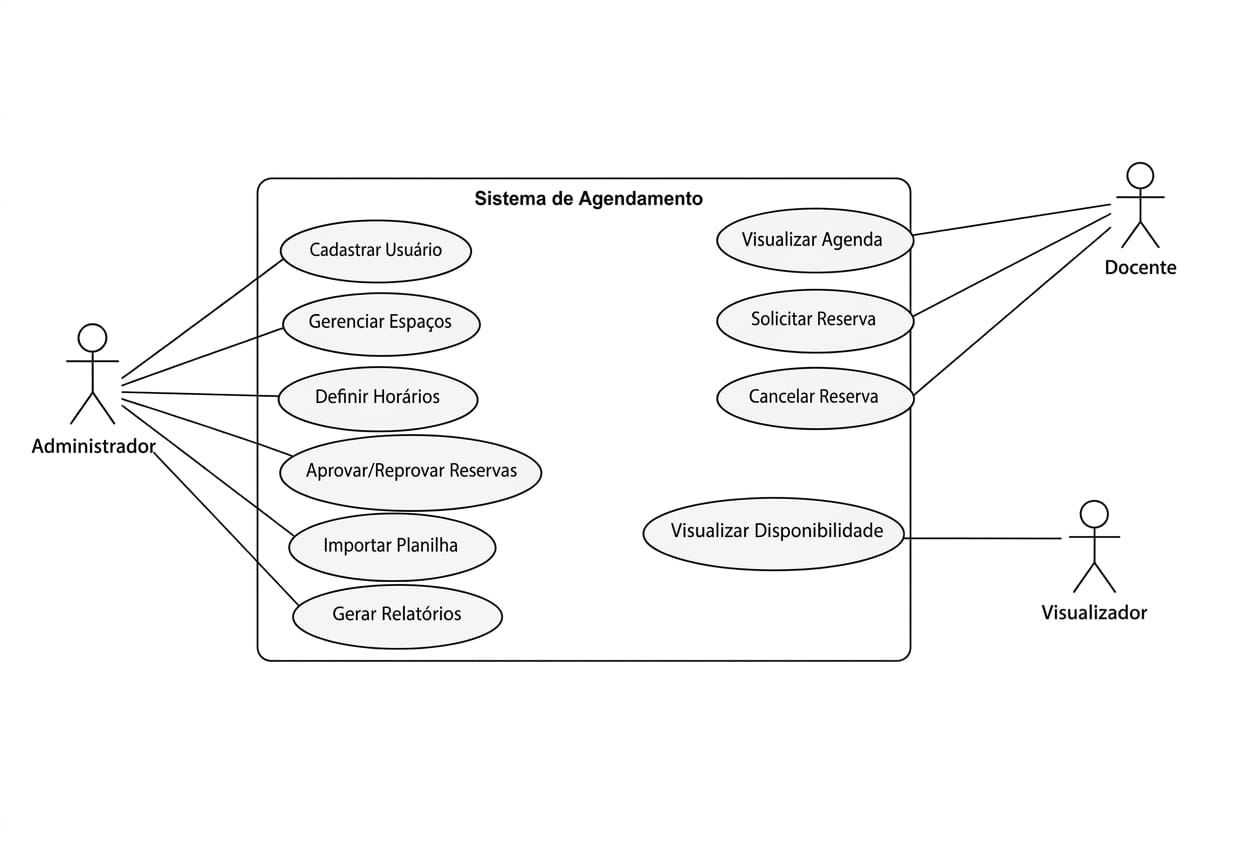
\includegraphics[width=0.95\textwidth, trim=10 165 10 140, clip]{Figuras/casos_de_uso}
    \caption*{Fonte: Elaborado pelo autor (2026).}
    \label{fig:casos_uso}
\end{figure}

O diagrama de classes será elaborado no TCC 2 e terá como entidades centrais do domínio \textit{EspaçoFísico}, \textit{Horário}, \textit{Solicitação}, \textit{Reserva} e \textit{Usuário}. Os relacionamentos entre essas entidades, como a associação entre \textit{Usuário} e \textit{Reserva} ou entre \textit{EspaçoFísico} e \textit{Horário}, definirão as regras de integridade que orientam a estrutura do banco de dados. \citeonline{larman2007} destaca que o diagrama de classes é o artefato de modelagem mais diretamente relacionado à estrutura do código, uma vez que suas entidades correspondem às classes que materializam o domínio na solução desenvolvida.

O diagrama de sequência, também previsto para o TCC 2, ilustrará como os objetos do sistema interagem ao longo do tempo para realizar uma operação. \citeonline{larman2007} aponta que esse artefato é útil para antecipar pontos de decisão e exceções no fluxo de execução, articulando a lógica das operações de solicitação e aprovação de reservas com as classes que compõem o domínio.

%-----------------------------------
\subsubsection{Implementação}
\label{sec:implementacao}

A quarta etapa é a implementação. Nesta fase do trabalho apresenta-se o seu planejamento, com a definição das tecnologias e da arquitetura, enquanto a codificação propriamente dita será realizada no TCC 2. O sistema será desenvolvido como uma aplicação web, com arquitetura e tecnologias definidas a seguir.

A linguagem de programação adotada é o Python, com o \textit{framework} Django, cujo padrão arquitetural MTV e funcionamento estão descritos nas Seções~\ref{sec:mvc_mtv} e~\ref{sec:django}. A escolha se justifica por reunir nativamente os componentes necessários ao sistema, o que reduz a dependência de bibliotecas externas e permite que o desenvolvimento se concentre nas regras de negócio, e pela separação entre dados, lógica e apresentação, que facilita a manutenção do código.

A Tabela~\ref{tab:funcionalidades} resume as funcionalidades do sistema, agrupadas pelos mesmos módulos dos requisitos funcionais.

\begin{table}[!htb]
	\centering
	\caption{Funcionalidades do sistema por módulo}
	\renewcommand{\arraystretch}{1.25}
	\newcommand{\fitem}[1]{\par\hangindent=1em\hangafter=1\noindent\makebox[1em][l]{\textbullet}#1}
	\begin{tabular}{@{}>{\raggedright\arraybackslash}p{4.0cm}>{\raggedright\arraybackslash}p{9.8cm}@{}}
	\hline
		\textbf{Módulo} & \textbf{Funcionalidades principais} \\ \hline
		Ensalamento & \fitem{Importação da planilha de horários, com prévia e confirmação}\fitem{Associação dos espaços da planilha aos já cadastrados}\fitem{Aulas recorrentes: alteração, encerramento e cancelamento de ocorrências} \\ \arrayrulecolor{black!25}\hline\arrayrulecolor{black}
		Espaços, cursos, disciplinas e turmas & \fitem{Cadastro e manutenção} \\ \arrayrulecolor{black!25}\hline\arrayrulecolor{black}
		Usuários e perfis & \fitem{Cadastro individual ou em lote (CSV)}\fitem{Definição e recuperação de senha}\fitem{Perfis com permissões definidas pelo superadministrador} \\ \arrayrulecolor{black!25}\hline\arrayrulecolor{black}
		Agenda de reservas & \fitem{Solicitação, inclusive em nome de outro usuário}\fitem{Análise: aprovação, rejeição ou sugestão de alternativa}\fitem{Acompanhamento das próprias solicitações} \\ \arrayrulecolor{black!25}\hline\arrayrulecolor{black}
		Notificações e comunicados & \fitem{Avisos em tempo real}\fitem{Comunicados para todos, para um perfil ou para usuários escolhidos} \\ \arrayrulecolor{black!25}\hline\arrayrulecolor{black}
		Consulta pública & \fitem{Calendário por data, com filtros por sala, docente, curso e turma}\fitem{Horário original da planilha}\fitem{Exportação do calendário (.ics)} \\ \arrayrulecolor{black!25}\hline\arrayrulecolor{black}
		Painel, relatórios e auditoria & \fitem{Painel de pendências e solicitações}\fitem{Mapa de ocupação por dia e horário}\fitem{Relatório de solicitações}\fitem{Registro das ações, sem alteração ou exclusão} \\ \arrayrulecolor{black!25}\hline\arrayrulecolor{black}
		Configurações & \fitem{Servidor de envio de e-mails configurado pela interface} \\ \arrayrulecolor{black!25}\hline\arrayrulecolor{black}
		Central de ajuda & \fitem{Tutoriais por tela, filtrados pelas permissões do usuário} \\ \hline
	\end{tabular}
	\label{tab:funcionalidades}
\end{table}

Para a camada de dados, será utilizado o PostgreSQL como sistema gerenciador de banco de dados relacional. A escolha se justifica frente a alternativas como o MySQL e o SQLite: embora o SQLite seja prático para ambientes de desenvolvimento, não é recomendado para aplicações com múltiplos acessos simultâneos em produção; o MySQL, por sua vez, é amplamente difundido, mas o PostgreSQL oferece maior conformidade com o padrão SQL, melhor tratamento de integridade referencial e suporte mais completo a transações complexas, recursos relevantes para a consistência das reservas. Soma-se a isso o suporte nativo e robusto do Django ao PostgreSQL, incluindo recursos como busca textual avançada e transações com alto nível de integridade \cite{djangodocs}. O acesso ao banco será feito exclusivamente por meio do ORM, mantendo consistência entre o código Python e o esquema relacional ao longo de todo o ciclo de desenvolvimento.

A camada de apresentação será construída com os \textit{templates} do Django combinados ao Tailwind CSS. Essa escolha agiliza o desenvolvimento da interface, mantém a consistência visual entre as telas e reduz o custo de manutenção, permitindo ajustes visuais sem alteração nas \textit{views} ou nos \textit{models}.

Para a autenticação dos usuários, será utilizada a biblioteca \textit{django-allauth}, escolhida por fornecer prontos os fluxos de registro, login, recuperação de senha e gerenciamento de sessões \cite{pennersr2024}. O controle de acesso descrito na Seção~\ref{sec:rbac} será implementado com perfis configuráveis. Cada permissão corresponde a uma ação sobre um recurso do sistema, como solicitar uma reserva ou editar um espaço, e o sistema define 47 permissões, distribuídas em 13 módulos. Um perfil é um conjunto dessas permissões, montado pelo superadministrador. Os perfis Administrador e Docente vêm na carga inicial apenas como exemplo e podem ser alterados. Outras categorias, como os técnicos administrativos, recebem um perfil com as permissões de que precisam. A verificação ocorre sempre no servidor, e a consulta pública dispensa autenticação.

As notificações automáticas serão exibidas no próprio sistema, em um ícone no cabeçalho que se atualiza em tempo real, sem recarregar a página (RNF11). Ao receber uma solicitação de reserva, o sistema notificará os responsáveis pela análise; após a decisão, o solicitante receberá o resultado (RF09 e RF10). O e-mail será usado apenas para a definição e a recuperação de senha, com o servidor de envio configurado pela interface (RF27) e as mensagens enviadas em segundo plano (RNF10) \cite{djangodocs}.

As notificações em tempo real serão implementadas com o Django Channels, extensão que permite ao Django manter conexões WebSocket com o navegador \cite{channelsdocs}. Tarefas demoradas, como a importação da planilha e o envio de e-mails, serão executadas por um processo próprio em segundo plano, que lê uma fila registrada no banco e repete o envio em caso de falha. A aplicação, o banco de dados e esse processo serão distribuídos em contêineres orquestrados pelo Docker Compose, o que facilita a implantação em ambientes diferentes \cite{dockerdocs}. 

O planejamento da implementação contempla ainda a definição da infraestrutura de hospedagem do sistema. Segundo a Diretora de Ensino Técnico, está em andamento uma articulação da direção do \textit{campus} com a FADETEC e com a Sifsoft, empresa júnior do curso de Bacharelado em Sistemas de Informação do \textit{campus} Salinas. Como essa articulação ainda não está concretizada, prevê-se, como alternativa, a hospedagem em plataformas gratuitas ou de baixo custo voltadas a aplicações web, a exemplo de Render, Railway ou PythonAnywhere, que oferecem suporte a aplicações Django e permitem disponibilizar o sistema sob um domínio público sem custo de infraestrutura para a instituição.

Cabe esclarecer o escopo deste ponto: o presente trabalho compreende o desenvolvimento e a disponibilização de uma versão funcional do sistema em ambiente acessível por navegador. A implantação definitiva na infraestrutura institucional ficará sob responsabilidade da direção do campus e pelos setores envolvidos.
%-----------------------------------
\subsubsection{Validação}
\label{sec:validacao}

A validação do sistema será feita por testes técnicos automatizados, unitários e de integração, conforme os conceitos da Seção~\ref{sec:testes}. Os testes serão escritos com o \textit{framework} de testes do Django, que executa cada caso sobre um banco de dados temporário \cite{djangodocs}, e cobrirão as regras de negócio críticas listadas na Tabela~\ref{tab:testes}. O critério de aceite é a execução de todos os testes sem falhas. A validação com usuários finais e a homologação institucional não fazem parte do escopo deste trabalho.

\begin{table}[!htb]
	\centering
	\caption{Regras de negócio verificadas pelos testes}
	\begin{tabular}{@{}>{\raggedright\arraybackslash}p{9.8cm}>{\raggedright\arraybackslash}p{4.0cm}@{}}
	\hline
		\textbf{Regra verificada} & \textbf{Requisitos} \\ \hline
		Bloqueio de reservas sobrepostas, inclusive em análises simultâneas & RF06, RF07, RNF08 \\
		Acesso a cada funcionalidade conforme as permissões do perfil & RF18, RNF01 \\
		Importação e reimportação da planilha de horários & RF01, RF02 \\
		Alteração, encerramento e cancelamento de aulas recorrentes & RF14--RF16 \\
		Envio das notificações ao solicitante e aos responsáveis & RF09, RF10 \\
		Consulta pública sem exposição de dados pessoais & RF11 \\
		Imutabilidade dos registros de auditoria & RF26, RNF09 \\ \hline
	\end{tabular}
	\label{tab:testes}
\end{table}

%---------------------------------
% SEÇÃO DE CRONOGRAMA
%---------------------------------
\section{Cronograma}
\label{sec:cronograma}

O cronograma da Tabela~\ref{tab:cronograma} contempla apenas a quarta e última etapa da pesquisa de implementação do sistema ao longo do segundo semestre de 2026. O desenvolvimento concentra-se entre agosto e novembro, de modo que a escrita e a entrega do TCC ocorram com a defesa, prevista para dezembro. As atividades foram distribuídas de forma a respeitar a dependência entre as camadas do sistema: a configuração do ambiente e a modelagem do banco de dados precedem o desenvolvimento das funcionalidades, que por sua vez antecedem os testes e os ajustes finais.

\begin{table}[!htb]
	\centering
	\caption{Cronograma de implementação -- 2º semestre de 2026}
	\resizebox{\textwidth}{!}{
		\begin{tabular}{@{}lccccc@{}}
		\hline
			\multicolumn{1}{c}{\multirow{2}{*}{\textbf{Etapa}}} & \multicolumn{5}{c}{\textbf{Meses}} \\
			\multicolumn{1}{c}{} &
			\multicolumn{1}{c}{Ago} &
			\multicolumn{1}{c}{Set} &
			\multicolumn{1}{c}{Out} &
			\multicolumn{1}{c}{Nov} &
			\multicolumn{1}{c}{Dez} \\ \hline
			Configuração do ambiente e estrutura do projeto & X &   &   &   &   \\
			Implementação dos \textit{Models} e banco de dados & X & X &   &   &   \\
			Desenvolvimento das \textit{Views} e roteamento de URLs &   & X &   &   &   \\
			Implementação dos \textit{Templates} e interface &   & X & X &   &   \\
			Autenticação e controle de acesso (RBAC) &   & X &   &   &   \\
			Módulo de importação de planilhas de horários &   &   & X &   &   \\
			Módulo de notificações em tempo real &   &   & X &   &   \\
			Geração de relatórios de uso &   &   &   & X &   \\
			Testes unitários e de integração &   &   & X & X &   \\
            Implantação em ambiente de hospedagem &   &   &   & X &   \\
			Ajustes finais e escrita do TCC 2 &   &   &   & X &   \\
			Defesa &   &   &   &   & X \\ \hline
		\end{tabular}
	}
	\label{tab:cronograma}
\end{table}

% ----------------------------------------------------------
% Referências bibliográficas
% ----------------------------------------------------------
\clearpage
\bibliography{referencias}
\end{document}
